\documentclass[conference]{IEEEtran}
\usepackage{mathptmx}
\usepackage{amsmath,amssymb,booktabs,graphicx,tikz}
\usepackage{balance}
\usepackage{algorithm}
\usepackage{algpseudocode}
\usepackage{url}
\usepackage[hidelinks]{hyperref}
\hypersetup{pdftitle={Recursive Boundary Retrieval for Long-Text Question Answering},pdfauthor={Veer Vikram Singh}}
\newcommand{\PilotCount}{10}
\newcommand{\EligibleCount}{109}
\newcommand{\MinimumWords}{2279}
\newcommand{\MaximumWords}{7293}
\newcommand{\RbrFone}{21.03}
\newcommand{\RbrCalls}{2.10}
\newcommand{\RbrTime}{10.81}
\newcommand{\DirectFone}{16.95}
\newcommand{\DirectCalls}{1.00}
\newcommand{\DirectTime}{31.72}
\newcommand{\BmFone}{22.49}
\newcommand{\BmCalls}{1.00}
\newcommand{\BmTime}{13.42}
\newcommand{\DenseFone}{26.18}
\newcommand{\DenseCalls}{1.00}
\newcommand{\DenseTime}{15.29}

\begin{document}
\title{Recursive Boundary Retrieval for Long-Text Question Answering}
\author{\IEEEauthorblockN{Veer Vikram Singh}}
\maketitle
\begin{abstract}
Finding a useful fact in a long document can be difficult for a language model. Earlier studies show that some models use information near the start or end of a context more reliably than information in its middle. This paper studies Recursive Boundary Retrieval (RBR), a simple method that checks short views of the outer thirds of a document. If neither view gives an answer, it removes those thirds and repeats the process on the middle. Nomic embeddings provide similarity scores, while a local model running through Ollama answers the question. A public-data pilot compares the original procedure with direct prompting, BM25, and dense retrieval. The work is ongoing. RBR can discard unseen evidence, stop on an incorrect answer, or fail when an answer needs information from several passages.
\end{abstract}
\begin{IEEEkeywords}
recursive boundary retrieval, long-context question answering, positional bias, retrieval evaluation
\end{IEEEkeywords}

\section{Introduction}
A user may paste a long report and ask for a particular date, name, instruction, or value. Sending the whole document to a model is simple, but it is limited by the context window and by how well the model uses the supplied text.

Liu et al. found that performance on their long-context tasks often depended on where useful information appeared. Information near the beginning or end was usually easier to retrieve than information in the middle \cite{liu}. RBR uses this observation as its motivation. After an unsuccessful check, it changes the input by removing the outer regions. Previously central material can then move closer to a boundary of the smaller input. This does not mean that every model has the same positional behavior.

The aim is to implement the original recursive procedure clearly and study its trade-offs. A small React application accepts pasted text and displays RBR beside direct prompting. A separate benchmark compares it with established retrieval methods. The study asks whether the recursive procedure can find specific information, how much work it uses, and where it fails.

\section{Related Work}
BM25 ranks passages through query-term matches, term frequency, and document-length normalization \cite{bm25}. Dense retrieval compares vector representations of questions and passages; Karpukhin et al. provide an important example \cite{dpr}. The dense baseline here uses general-purpose Nomic embeddings, not the trained DPR model. Nomic specifies separate query and document prefixes for retrieval inputs \cite{nomic}.

RBR follows document position rather than a relevance-ranked search path. Embeddings do not select the next third. Its motivation comes from positional effects \cite{liu}, but the pilot does not separate those effects from the benefit of shorter inputs. LongBench provides public long-context tasks and reference answers for evaluation \cite{longbench}.

\section{Methodology}
\subsection{Recursive Boundary Checks}
Represent the document as $D=(w_1,\ldots,w_N)$ and the question as $q$. At depth $d$, divide the current region $R_d$ into left, middle, and right thirds, denoted $L_d$, $M_d$, and $U_d$. Integer remainders stay in the right third.

For boundary width $b=400$, a third $B$ is presented as
\begin{equation}
V_b(B)=\begin{cases}
B,&|B|\leq 2b,\\
B[1:b]\Vert B[|B|-b+1:|B|],&|B|>2b.
\end{cases}
\end{equation}
The join operator inserts an omission marker between separate excerpts. This avoids making the excerpts appear adjacent in the source.

The model checks $V_b(L_d)$ first. If it returns \texttt{NOT\_FOUND}, the model checks $V_b(U_d)$. If both checks fail, RBR removes the outer thirds and continues with
\begin{equation}
R_{d+1}=M_d.
\end{equation}
It stops when an answer is returned, the region has at most 500 words, or depth eight is reached. At either size or depth limit, the remaining core is evaluated in full with notes from the last five unsuccessful views.

\begin{figure}[t]
\centering
\resizebox{\columnwidth}{!}{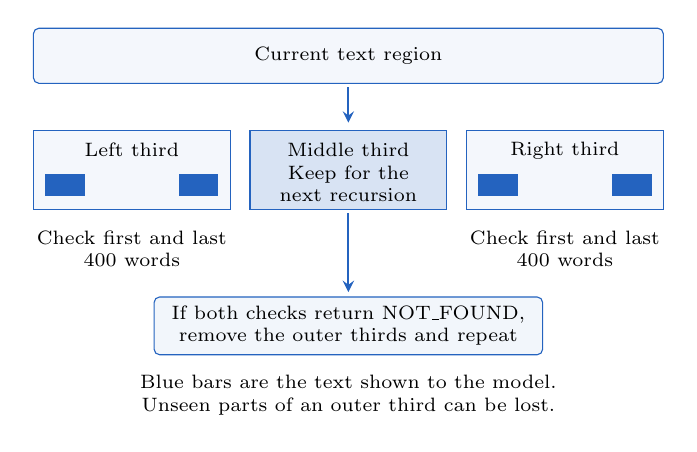
\begin{tikzpicture}[x=1cm,y=1cm,font=\scriptsize,>=stealth]
\definecolor{rbrblue}{RGB}{36,99,191}
\draw[draw=rbrblue,fill=rbrblue!5,rounded corners=2pt] (0,0) rectangle (8,0.7);
\node at (4,0.35) {Current text region};
\draw[->,rbrblue,thick] (4,-0.05) -- (4,-0.5);
\draw[draw=rbrblue,fill=rbrblue!5] (0,-1.6) rectangle (2.5,-0.6);
\draw[draw=rbrblue,fill=rbrblue!18] (2.75,-1.6) rectangle (5.25,-0.6);
\draw[draw=rbrblue,fill=rbrblue!5] (5.5,-1.6) rectangle (8,-0.6);
\node at (1.25,-0.85) {Left third};
\node at (4,-0.85) {Middle third};
\node at (6.75,-0.85) {Right third};
\foreach \position in {0.15,1.85,5.65,7.35} {\fill[rbrblue] (\position,-1.43) rectangle +(0.5,0.28);}
\node[align=center] at (4,-1.28) {Keep for the\\next recursion};
\node[align=center] at (1.25,-2.1) {Check first and last\\400 words};
\node[align=center] at (6.75,-2.1) {Check first and last\\400 words};
\draw[->,rbrblue,thick] (4,-1.65) -- (4,-2.65);
\node[draw=rbrblue,rounded corners=2pt,fill=rbrblue!6,align=center,text width=4.7cm] at (4,-3.08) {If both checks return NOT\_FOUND,\\remove the outer thirds and repeat};
\node[align=center,text width=7.6cm] at (4,-3.96) {Blue bars are the text shown to the model.\\Unseen parts of an outer third can be lost.};
\end{tikzpicture}
}
\caption{The original procedure. Outer views are checked in order; the middle is retained only after both return no answer.}
\label{fig:process}
\end{figure}

\subsection{Embeddings and the Decision Rule}
RBR divides each outer third into 256-word chunks. With embedding function $E$, its recorded similarity is
\begin{equation}
S(q,B)=\max\left(\{0\}\cup\left\{\cos(E(q),E(c)):c\in\mathcal C(B)\right\}\right).
\end{equation}
Here $\mathcal C(B)$ is the set of chunks in $B$. Max-pooling keeps the strongest local match rather than averaging all chunk vectors. However, similarity alone does not establish that a region contains an answer.

Both outer scores are computed before the answer checks. As in the original implementation, these scores are diagnostic: they do not change the left-first order, choose the middle, or decide when to stop. The query is embedded once per request, and identical chunks can reuse embeddings. These small changes reduce repeated work without changing the recursive path.

A nonempty model response that does not start with \texttt{NOT\_FOUND} is accepted. This is a binary response check, not a calibrated confidence probability. A cosine score must therefore not be read as answer confidence.

\begin{algorithm}[t]
\caption{Recursive Boundary Retrieval}
\begin{algorithmic}[1]
\Require Region $R$, question $q$, depth $d$, notes $H$
\If{$|R|\leq500$ or $d\geq8$}
\State \Return Answer$(q,R,\operatorname{LastFive}(H))$
\EndIf
\State $(L,M,U)\gets\operatorname{SplitThree}(R)$
\State Compute $S(q,L)$ and $S(q,U)$
\For{$B$ in $(L,U)$, in order}
\State $a\gets\operatorname{Answer}(q,V_{400}(B))$
\State Record the score, excerpts, and response
\If{$a$ is nonempty and not \texttt{NOT\_FOUND}}
\State \Return $a$
\EndIf
\State Append an unsuccessful-view note to $H$
\EndFor
\State \Return RBR$(M,q,d+1,H)$
\end{algorithmic}
\end{algorithm}

\subsection{Cost and Coverage}
Without early stopping, region size decreases by roughly a factor of three per level. Ignoring integer rounding, the number of split levels is
\begin{equation}
\ell\approx\min\left\{8,\max\left(0,\left\lceil\log_3\frac{N}{500}\right\rceil\right)\right\}.
\end{equation}
There are at most $2\ell+1$ answer-model calls. Outer views contain at most $4b\ell$ document words in total, followed by a core of length $C$. Separators and instructions add further tokens; words are not model tokens.

This is not an $O(\log N)$ claim for total retrieval work. The outer thirds are embedded before they are discarded. Their sizes form a geometric sum of order $N$ during a complete unsuccessful search. Embedding, text processing, and inference all contribute to cost.

RBR also has no general coverage guarantee. In a 21,000-word document, the left third contains about 7,000 words. A fact near word 2,000 is outside its first and last 400 words. The model never sees the fact, but the third can still be removed. Even a perfect evaluator would miss that position. Figure~\ref{fig:process} distinguishes a third from its visible ends.

\subsection{Application}
The backend uses Python and FastAPI, and the frontend uses React and JavaScript. Both models run locally through Ollama. Text is kept in request memory rather than a document database. The interface accepts pasted text or a UTF-8 text file, then displays the two answers with elapsed time, answer-call counts, processed prompt tokens, and embedding requests. Each RBR trace step includes its depth, side, word positions, similarity, and actual excerpts. The methods run sequentially to avoid competing for the same local model. Interface and HTTP overhead are not included in the benchmark's method timings.

\section{Dataset and Experimental Setup}
The pilot uses the public English MultiFieldQA part of LongBench \cite{longbench}. The code downloads a public JSONL mirror and verifies its SHA-256 checksum. The inclusion rule keeps contexts with 2,000--8,000 whitespace-separated words. From \EligibleCount{} eligible examples, \PilotCount{} were sampled with seed 2026. Their observed lengths are \MinimumWords{}--\MaximumWords{} words. This subset is not an official leaderboard evaluation.

The generator is local \texttt{llama3.2}, and embeddings use \texttt{nomic-embed-text}. The run used Ollama 0.24.0 on an Apple M2 machine with 16 GiB of memory. Every method uses the same basic answer instructions, temperature zero, generation seed 42, a 32,768-token context setting, and a 256-token output limit. Direct prompting sends the entire document once. BM25 and dense retrieval select up to eight overlapping 256-word passages, with a 48-word overlap, and restore document order before generating once. RBR's final core additionally receives its inspection notes.

Method order is randomized within each question, after a warm-up. The saved record includes model digests, dataset and source hashes, question IDs, token counts, embedding time, total time, and call counts. Client caches are separate between methods. Total method time includes embedding and scoring. Local model loading and service caching can still affect timing.

Answer quality uses best-reference normalized token F1 and exact match. Normalization removes case, punctuation, and English articles. For token multisets $P$ and $G$,
\begin{equation}
F_1=\frac{2|P\cap G|}{|P|+|G|},
\end{equation}
with empty inputs handled separately. F1 measures word overlap, not evidence support. Paired bootstrap intervals are saved to describe uncertainty. RBR may make several calls, so total input and call budgets are not matched.

\balance
\section{Pilot Results}
\begin{table}[t]
\caption{Pilot results. F1 and calls are means; time is median total method time, including embeddings.}
\label{tab:results}
\centering
\begin{tabular}{lrrr}\toprule
Method & F1 (\%) & Calls & Time (s)\\\midrule
RBR & \RbrFone & \RbrCalls & \RbrTime\\
Direct prompting & \DirectFone & \DirectCalls & \DirectTime\\
BM25 & \BmFone & \BmCalls & \BmTime\\
Dense retrieval & \DenseFone & \DenseCalls & \DenseTime\\\bottomrule
\end{tabular}
\end{table}
Table~\ref{tab:results} reports fresh measurements; no older prototype score is reused. Per-question predictions are retained in the results file. The small sample cannot establish a stable ranking. Differences can reflect evidence selection, repeated answer attempts, or generation behavior rather than positional bias alone.

RBR obtained \RbrFone\% mean F1, compared with \DirectFone\% for direct prompting. BM25 and dense retrieval obtained \BmFone\% and \DenseFone\%, respectively. RBR therefore improved on direct prompting in this sample but did not lead the passage-retrieval baselines. Its median total time was \RbrTime{} seconds, compared with \DirectTime{} seconds for direct prompting. Shorter prompts can reduce cost even when several calls are made; this observation does not prove that positional bias caused the difference. No method achieved normalized exact match in this pilot.

A deterministic regression test also places a fact in an unviewed outer-third interior. RBR misses it while a full-text oracle can see it. This tests coverage geometry, not language-model accuracy. Other tests cover recursion order, early stopping, the final core, embedding prefixes, and direct prompting.

\section{Drawbacks and Ongoing Research}
A negative answer about a short view does not establish that the whole third is irrelevant. Early acceptance can also return an unsupported answer. Questions that need several passages are difficult because the separate views may never supply all required facts together.

The recorded embedding scores do not fix these problems because they are not used for routing or verification. Embedding much of the text can make RBR slow even when its answer prompts are short. Direct prompting has a different limit: sending the full document does not ensure that all its tokens fit. The interface shows processed tokens and warns about possible context truncation, which Ollama does not report exactly.

The current evaluation uses one generator, one embedding model, and a small English sample. It does not establish superiority. More questions, document lengths, models, and annotated supporting passages are needed. Equal-total-token and equal-call comparisons would help measure the quality/cost trade-off. A focused follow-up could keep the evidence fixed and change only its prompt position, testing the boundary motivation more directly without changing the original recursive rule.

\section{Conclusion}
RBR offers a simple way to expose progressively central parts of a long text. This implementation preserves the original outer-view checks and middle-third recursion, with embedding scores shown for inspection. The pilot and failure tests provide a starting point for further study. The method remains imperfect: it can discard unseen evidence and accept a wrong answer. Larger controlled experiments are needed before making stronger claims.

\begin{thebibliography}{00}
\bibitem{liu} N. F. Liu et al., ``Lost in the middle: How language models use long contexts,'' \emph{Transactions of the Association for Computational Linguistics}, vol. 12, pp. 157--173, 2024, doi: 10.1162/tacl\_a\_00638.
\bibitem{bm25} S. Robertson and H. Zaragoza, ``The probabilistic relevance framework: BM25 and beyond,'' \emph{Foundations and Trends in Information Retrieval}, vol. 3, no. 4, pp. 333--389, 2009, doi: 10.1561/1500000019.
\bibitem{dpr} V. Karpukhin et al., ``Dense passage retrieval for open-domain question answering,'' in \emph{Proceedings of EMNLP}, 2020, pp. 6769--6781, doi: 10.18653/v1/2020.emnlp-main.550.
\bibitem{nomic} Nomic AI, ``nomic-embed-text-v1.5,'' model card. [Online]. Available: \url{https://huggingface.co/nomic-ai/nomic-embed-text-v1.5}. Accessed: Nov. 17, 2026.
\bibitem{longbench} Y. Bai et al., ``LongBench: A bilingual, multitask benchmark for long context understanding,'' in \emph{Proceedings of ACL}, 2024, pp. 3119--3137, doi: 10.18653/v1/2024.acl-long.172.
\end{thebibliography}
\end{document}
